\section*{Ziel}
Ziel ist es, mit den Eigenschaften von Ultraschall vertraut zu werden und den Umgang damit zu erlernen. Es wird Schallgeschwindigkeit $c$ in Acryl bestimmt, ein Acrylblock auf Materialfehler untersucht und die Abmessungen eines Augenmodells bestimmt.

\section{Theorie}
\label{sec:Theorie}
Schall bewegt sich in Form von Druckschwankungen als longitudinale Welle
\begin{equation}
p(x,t)=p_o+v_oZ\cos{(\omega t - kx)}
\label{eq:long_welle}
\end{equation}
durch ein Medium. Dabei ist $Z=c\cdot\rho$ die von der Materialdichte abhängige akustische Impedanz und $c$ die richtungs- und materialabhängige Schallgeschwindigkeit. Einfluss auf die Schallgeschwindigkeit nehmen die Kompressibilitätszahl $\kappa$ in Flüssigkeiten und der Elastizitätsmodul $E$ in Festkörpern. Es gilt
\begin{align}
c_\mathup{Fl}=\sqrt{\frac{1}{\kappa\rho}}\quad, &\qquad c_\mathup{F_e}=\frac{E}{\rho}.
\label{eq:schallgeschwindigkeit}
\end{align}
Durch die Druckschwankungen innerhalb des Materials treten Reibungseffekte auf, die zu einem Energieverlust des Schalls und damit zu einer Intensitätsabnahme führen. Je tiefer der Schall eindringt, desto geringer wird diese. Es gilt
\begin{equation}
I(x)=I_0\cdot\mathup{e}^{\alpha x}
\label{eq:intensitaet}
\end{equation}
mit dem negativen Absorptionskoeffizienten $\alpha$.
Schall bestizt die typischen Eigenschaften einer Welle und wird beispielsweise an Grenzflächen reflektiert. Dabei ist der Reflexionskoeffizient
\begin{equation}
R=\left(\frac{Z_1-Z_2}{Z_1+Z_2}\right)².
\label{eq:reflexion}
\end{equation}
Menschen besitzen die Fähigkeit Geräusche wahrzunehmen, deren Frequenz sich zwischen $\SI{16}{\hertz}$ und $\SI{20}{\kilo\hertz}$ befindet. Ultraschall mit  $\SI{20}{\kilo\hertz}$ - $\SI{1000}{\kilo\hertz}$ liegt in einem nicht wahrnehmbaren Frequenzbereich. Die Eigenschaften des Schalls lassen sich in der Medizin oder Materialprüfungen ausnutzen. Dabei wird der Ultraschall mit dem reziproken piezo-elektrischen Effekt erzeugt. Ein piezo-Kristall, beispielsweise Quarz, wird in ein elektrisches Wechselfeld gebracht und zu Schwingungen angeregt. Diese Schwingungen werden in Form von Ultraschallwellen abgestrahlt. Der Effekt lässt sich jedoch nicht nur ausnutzen, um Ultraschall zu erzeugen. Er kann ebenfalls eingesetzt werden, um den Schall zu detektieren. Wird der Kristall durch Ultraschall zum Schwingen angeregt lässt sich ein elektrisches Signal abgreifen. Um nun Materialien zu untersuchen bestehen verschiedene Möglichkeiten der Laufzeitmessung. 
\begin{figure}
\centering
\begin{subfigure}{0.48\textwidth}
\centering
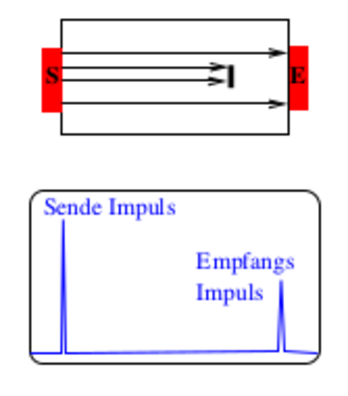
\includegraphics[height=5cm]{Bilder/Durchschallung.pdf}
\caption{Duchschallungsverfahren.}
\label{fig:durchschallung}
\end{subfigure}
\begin{subfigure}{0.48\textwidth}
\centering
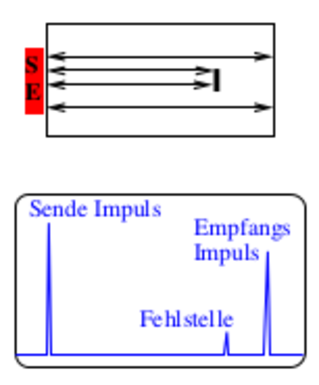
\includegraphics[height=5cm]{Bilder/Impuls-Echo.pdf}
\caption{Impuls-Echo-Verfahren}
\label{fig:impuls-echo}
\end{subfigure}
\caption{Zwei Verfahren der Materialuntersuchung.}%\cite{skript}}
\label{fig:verfahren}
\end{figure}
\begin{itemize}
\item Durchschallungsverfahren

Der zu untersuchende Gegenstand befindet sich zwischen zwei Sonden. Der Sender schickt den Schall durch den Körper, der Empfänger detektiert ihn. Trifft der Schall dabei auf einen Materialfehler wird von dem Empfänger eine Intensität gemessen die geringer ist als der nach Gleichung \eqref{eq:intensitaet} erwartete Wert. Nachteil dieses Verfahrens ist, dass keine Aussage über den Ort des Materialfehlers getroffen werden kann.
\item Impuls-Echo-Verfahren

Hier wird eine Sonde benötigt, die gleichzeitig Sender und Empfänger darstellt. Trifft der Schall nun auf die fehlerhafte Stelle wird er reflektiert, während der restliche Schall weiter durch den Körper läuft. Durch bestimmten der Laufzeit $\Delta{t}$ kann die Lage des Fehlers über
\begin{equation}
s=\frac{1}{2}ct
\label{eq:laufzeit}
\end{equation}
gefunden werden.
\end{itemize}
Desweiteren wird zwischen A- und B-Scan unterschieden. Der Amplituden-Scan ist ein 1-dimensionales Verfahren und wird zum Abtasten der Materialstruktur genutzt. Dabei wird die Amplitude als Funktion der Laufzeit $t$ aufgetragen. Der Brightness-Scan liefert ein 2-dimensionales Schnittbild, indem die reflektierten Amplituden als Helligkeitsabstufungen aufgetragen werden. Die Sonde muss dabei über den Körper geführt werden.
